\documentclass[a4paper, 10pt]{article}

\usepackage[english]{babel}
\usepackage[T1]{fontenc}
\usepackage[utf8]{inputenc}
\usepackage{textcomp}
\setlength{\marginparwidth}{2cm}

\usepackage{comment}
\usepackage{todonotes}

\usepackage{amsmath}
\usepackage{amssymb}
\usepackage{bm}

\usepackage{enumitem}
\usepackage{array}
\setlength\extrarowheight{5pt}

\usepackage{xcolor}
\usepackage{graphicx}
\graphicspath{ {./img/} }

\usepackage{hyperref}
\usepackage{listings}
\usepackage{color}
\definecolor{dkgreen}{rgb}{0,0.6,0}
\definecolor{gray}{rgb}{0.5,0.5,0.5}
\definecolor{mauve}{rgb}{0.58,0,0.82}
\lstset{frame=tb,
    language=Python,
    aboveskip=3mm,
    belowskip=3mm,
    showstringspaces=false,
    columns=flexible,
    basicstyle={\small\ttfamily},
    numbers=none,
    numberstyle=\tiny\color{gray},
    keywordstyle=\color{blue},
    commentstyle=\color{dkgreen},
    stringstyle=\color{mauve},
    breaklines=true,
    breakatwhitespace=true,
    tabsize=3
}

\title{Homework Assignment N°4}
\author{BML36\\Thibault Douzon\\Rajavarman Mathivanan}
\date{October 3rd, 2018}

\begin{document}
\maketitle

\pagebreak

\tableofcontents

\pagebreak
\section{Exercise 1: NN 1-D output}
\subsection{Part a}

\section{Exercise 2: NN 2-D output}
\subsection{Part a}
The neural network described in this exercise could be represented like this.
\begin{center}
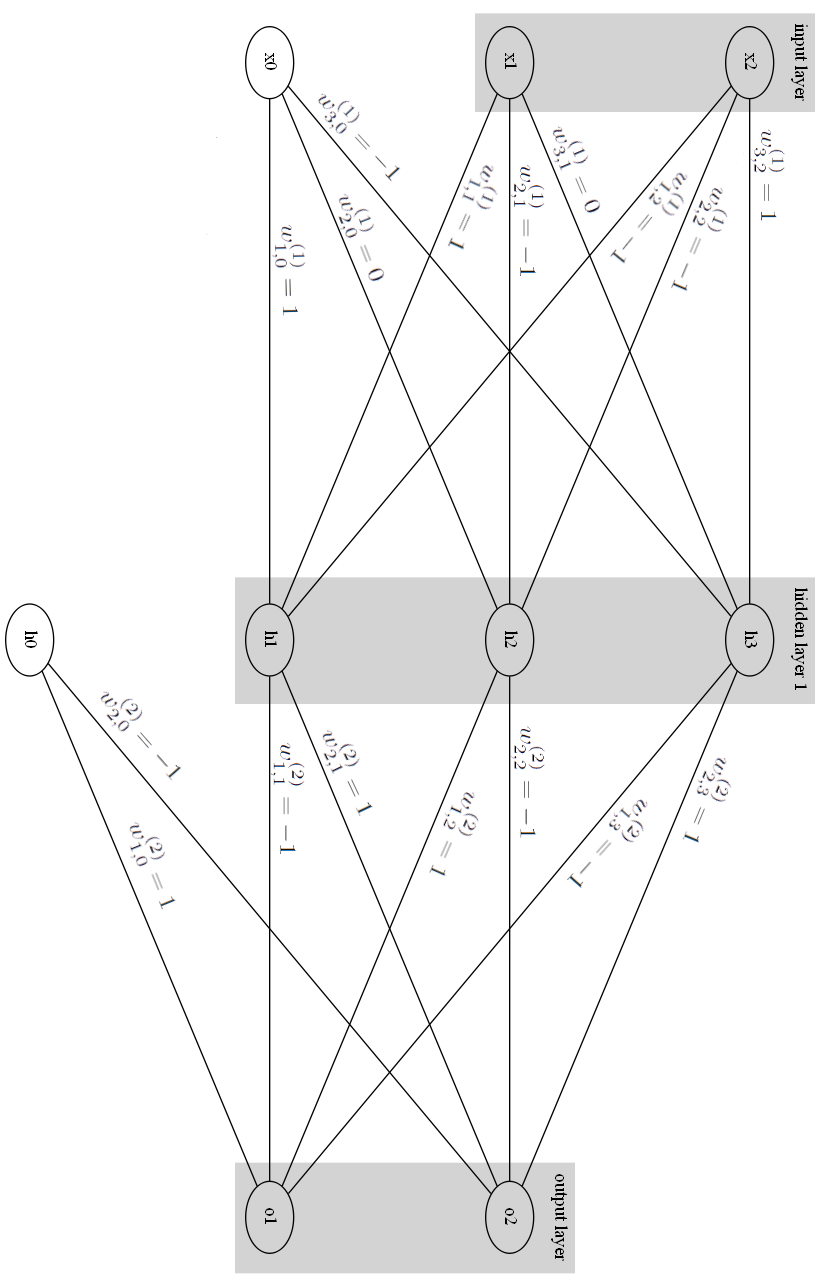
\includegraphics[scale=0.5]{ex2_graph_export}
\end{center}
It is structured in 3 parts: the input layer first (denoted $x1$, $x2$), then the hidden layer
(denoted $h1$, $h2$ and $h3$) and then the output layer (denoted $o1$ and $o2$).
\\
Nodes with indice 0 represent the bias introducted into the model.
\\ 
Each arc carries the value of the weight (denoted $w_{k,j}^{(l)}$ where $l$ is the layer, $k$ is the destination node
and $j$ is the origin node which lies in the layer $l-1$).

To compute the output of the neural network, we need to propagate
through the network the values of the input. Hidden layer applies a sigmoïd activation function
and output neurons have a linear activation function (identity function).
\\
Thus we can first compute every $a_k^{(1)}$, the signal recieved by each node in the hidden layer.
It is easier to make this computation under matrix representation, let's introduce the input vector $X$ and
the weights of the first layer $W^{(1)}$:
$$
X = [a_i^{(0)}] = [x_i] =\begin{bmatrix}
    1\\
    1\\
    1
\end{bmatrix}
$$
$$
W^{(1)} = [w_{j,i}^{(1)}] =  \begin{bmatrix}
    1 & 0 & -1\\
    1 & -1 & 0\\
    -1 & -1 & 1
\end{bmatrix}
$$
The signal recieved by the hidden layer is given by the following formula:
$$
H_{j\ne0} = [a_j^{(1)}]_{j\ne0} = X^\top W^{(1)} = \begin{bmatrix}
    1\\
    -2\\
    0
\end{bmatrix}
$$
Before repeating the same procedure, we need to apply the activation function
to each recieved signal and then concatenate the bias.
\\
The hidden layer uses the sigmoïd function as activation:
$$
\sigma(H_{j\ne0}) = [\sigma(a_j{(1)})] = \begin{bmatrix}
    \sigma(1)\\
    \sigma(-2)\\
    \sigma(0)
\end{bmatrix}
\approx \begin{bmatrix}
        0.731\\
        0.119\\
        0.5
\end{bmatrix}
$$
Now we can concatenate the bias at the beginning with a fixed value of 1:
$$
H_{out} \approx \begin{bmatrix}
    1\\
    0.731\\
    0.119\\
    0.5
\end{bmatrix}
$$
The vector $H_{out}$ is the signed emitted by the hidden layer.
\\
We can now repeat the same procedure with the second layer with $H_{out}$ as input and 
use the weights of the output layer.
\\
The weights of the second layer are the following:
$$
W^{(2)} = [w_{k,j}^{(2)}] = \begin{bmatrix}
    1 & -1\\
    -1 & 1\\
    1 & -1\\
    -1 & 1
\end{bmatrix}
$$
And we can compute the signal recieved by the output layer:
$$
O = [a_k^{(2)}] = {H_{out}}^\top W^{(2)} \approx \begin{bmatrix}
    -0.112\\
    0.112
\end{bmatrix}
$$
This is the output of our neural network as the activation
fonction of the output neuron is the identity function.

\subsection{Part b}
The formula to compute $\delta_i^{(l)}$ is the following:
$$
\delta_i^{(l)} = \frac{\partial E_n}{\partial a_i^{(l)}}
$$
Where $l$ is the layer and $i$ is the index of the neuron.
\\
But to compute the value of this expression for different values of $l$ and $i$,
we need to know the expression of $E_n$ first. $E_n$ is the error of the network
on the data sample number $n$. It is defined as follows:
$$
E_n(w) = \frac{1}{2} \sum_{k=1}^D ( y_k(x_n,w)-t_{n,k})^2
$$
Where $N$ is the number of output neurons (in our case 2), $x_n$ the input data and 
$t_n$ the target related to $x_n$, $w$ the current weigths of the neural network and 
$y_k$ the function that computes the $k^\text{th}$ coordinate of the NN's prediction based on the input data.
\\
In our case, we can rewrite this expression to this:
$$
E_n(w) = \frac{1}{2} \sum_{k=1}^2( y_k(x_n, w)-t_{n,k})^2
$$
And because the activation function of the output layer is the identity function,
we also have the following equation:
$$
y_k(x_n,w) = h(a_k^{(2)}) = a_k^{(2)}
$$
The analytical expressions of $\delta_1^{(2)}$ and $\delta_2^{(2)}$ directly follows:
$$
\delta_i^{(2)} = \frac{\partial E_n}{\partial a_i^{(2)}} = \frac{1}{2}\frac{\partial  \sum_{k=1}^2( a_k^{(2)}-t_{n,k})^2}{\partial a_i^{(2)}} = a_i^{(2)} - t_{n,i}
$$
We finally get the following numerical values:
$$
\delta_1^{(2)} = a_1^{(2)} - t_{n,1} = -0.112 - 1 = -1.112
$$
$$
\delta_2^{(2)} = a_2^{(2)} - t_{n,2} = 0.112 - (-1) = 1.112
$$

\subsection{Part c}
The formula to update a weight is the same as in previous models:
$$
w^{[\tau +1]} = w^{[\tau]} - \eta \frac{\partial E_n}{\partial w}(w^{[\tau]})
$$
We can use it to compute the new value of weight $w_{2,1}^{(2)}$ 
\\
First we will focus on computing $\frac{\partial E_n}{\partial w_{2,1}^{(2)}}$:
$$
\frac{\partial E_n}{\partial w_{2,1}^{(2)}}(w) = \frac{\partial E_n}{\partial a_2^{(2)}} \cdot \frac{\partial a_2^{(2)}}{\partial w_{2,1}^{(2)}}(w)
$$
$$
\frac{\partial E_n}{\partial w_{2,1}^{(2)}}(w) = \delta_2^{(2)} \cdot \frac{\partial a_2^{(2)}}{\partial w_{2,1}^{(2)}}(w) 
$$
From our previous computation in part a, we know the formula for $a_2^{(2)}$:
$$
a_2^{(2)} = \sum_{i=1}^3 w_{2,i}^{(2)}\sigma(a_i^{(1)}) + w_{(2,0)}^{(2)}
$$
Hence we deduce:
$$
\frac{\partial a_2^{(2)}}{\partial w_{2,1}^{(2)}}(w) = \sigma(a_1^{(1)}) \approx 0.731
$$
And finally we get:
$$
\frac{\partial E_n}{\partial w_{2,1}^{(2)}}(w) = \delta_2^{(2)} \cdot \frac{\partial a_2^{(2)}}{\partial w_{2,1}^{(2)}}(w) \approx 1.112 \times 0.731 \approx 0.813 
$$
We can now apply the formula to update the weight for $w_{2,1}^{(2)}$:
$$
w_{2,1}^{(2)[2]} = w_{2,1}^{(2)[1]} - \eta \frac{\partial E_n}{\partial w_{2,1}^{(2)}}(w_{2,1}^{(2)[1]}) 
$$
$$
w_{2,1}^{(2)[2]} \approx 1 - 0.5 \times 0.813 \approx 0.594
$$
When applying backpropagation with learning rate of 0.5, the new value of $w_{2,1}^{(2)}$ is 0.594
\subsection{Part d}
The first formula from part b still stands:
$$
\delta_i^{(l)} = \frac{\partial E_n}{\partial a_i^{(l)}} = \sum_k \frac{\partial E_n}{\partial a_k^{(l+1)}}\frac{\partial a_k^{(l+1)}}{\partial a_i^{(l)}}
$$
Thus in our case:
$$
\delta_2^{(1)} = \frac{\partial E_n}{\partial a_2^{(1)}} = \sum_{k=1}^2 \frac{\partial E_n}{\partial a_k^{(2)}}\frac{\partial a_k^{(2)}}{\partial a_2^{(1)}}
$$
Now because $a_Z^{(1)}$ takes part in every output node, we need to sum over all contributions to the output nodes.
Moreover, because the hidden layer does not use the identity function as activation, we need to take into account the contribution
of the activation funtion. This means we need to use the following formula from the lecture:
$$
\delta_j^{(l)} = h^\prime(a_j^{(l)})\sum_k w_{k,j}^{(l+1)}\delta_k^{(l+1)} 
$$
Which gives in our case:
$$
\delta_2^{(1)} = \sigma^\prime(a_2^{(1)})\sum_{k=1}^2 w_{k,2}^{(2)}\delta_k^{(2)} 
$$
Using the fact that $\sigma^\prime(x) = \sigma(x)(1-\sigma(x))$ we can rewrite it:
$$
\delta_2^{(1)} = \sigma(a_2^{(1)})(1-\sigma(a_2^{(1)}))\sum_{k=1}^2 w_{k,2}^{(2)}\delta_k^{(2)} 
$$
$$
\delta_2^{(1)} \approx 0.119\cdot(1-0.119)\times [1\cdot(-1.112)+(-1)\cdot1.112] \approx -0.233
$$
During the first backpropagation, the value of $\delta_2^{(1)}$ is roughly $-0.233$
\subsection{Part e}
In this part we want to compute the weights of the neuron 2 of the hidden layer, $\forall k \in \{0,1,2\}, w_{2,k}^{(1)}$ in a more precise way 
\\
This is very similar to part c, we need to update some weights so we will use the same formula:
$$
w^{[\tau +1]} = w^{[\tau]} - \eta \frac{\partial E_n}{\partial w}(w^{[\tau]})
$$
Where we can use the following formula to compute the gradient:
$$
\frac{\partial E_n}{\partial w_{2,k}^{(1)}}(w) = \delta_2^{(1)} \cdot \frac{\partial a_2^{(1)}}{\partial w_{2,k}^{(1)}}(w),  \forall k\in\{0,1,2\} 
$$
And the term $\frac{\partial a_2^{(1)}}{\partial w_{2,k}^{(1)}}(w)$ can be simplified like this:
$$
\frac{\partial a_2^{(1)}}{\partial w_{2,k}^{(1)}}(w) = x_k, \forall k \in\{0,1,2\}
$$
Where $x_k$ is the $k^\text{th}$ coordinate of the input. To simplify the notation, it uses the convention that says $x_0=1$ to
include the bias inside the input vector.
\\
Now we are prepared to replace each term with its value for every weight wwe want to update:
$$
w_{2,k}^{(1)[\tau +1]} = w_{2,k}^{(1)[\tau]} - \eta \delta_2^{(1)}x_k, \forall k \in \{0,1,2\}
$$
For $w_{2,0}^{(1)}$:
$$
w_{2,0}^{(1)[2]} = w_{2,0}^{(1)[1]} - \eta \delta_2^{(1)}x_0
$$
$$
w_{2,0}^{(1)[2]} \approx 0 - 0.5\cdot(-0.233)\cdot1 \approx 0.117
$$
For $w_{2,1}^{(1)}$:
$$
w_{2,1}^{(1)[2]} = w_{2,1}^{(1)[1]} - \eta \delta_2^{(1)}x_1
$$
$$
w_{2,1}^{(1)[2]} \approx (-1) - 0.5\cdot(-0.233)\cdot1 \approx -0.884
$$
For $w_{2,2}^{(1)}$:
$$
w_{2,2}^{(1)[2]} = w_{2,2}^{(1)[1]} - \eta \delta_2^{(1)}x_2
$$
$$
w_{2,2}^{(1)[2]} \approx (-1) - 0.5\cdot(-0.233)\cdot1 \approx -0.884
$$
\end{document}
    
$$
\frac{\partial E}{\partial w_i}(w) = \frac{\partial \frac{1}{2}\sum_{n=1}^N (\sigma(w^\top x_n) - t_n)^2}{\partial w_i}
$$
$$
\frac{\partial E}{\partial w_i}(w) =\sum_{n=1}^N \frac{\partial \frac{1}{2} (\sigma(w^\top x_n) - t_n)^2}{\partial \sigma(w^\top x_n)-t_n} \cdot \frac{\partial \sigma(w^\top x_n)-t_n}{\partial w^\top x_n}\cdot \frac{\partial w^\top x_n}{\partial w_i}
$$
$$
\frac{\partial E}{\partial w_i}(w) =\sum_{n=1}^N (\sigma(w^\top x_n)-t_n) \cdot \sigma(w^\top x_n)(1-\sigma(w^\top x_n)) \cdot x_{n,i}
$$

$$
\frac{A}{B} = \frac{A}{D}\times\frac{D}{C}\times\frac{C}{B}
$$

$$
E(w) = \frac{1}{2}\sum_{n=1}^N (\sigma(w^{(1)}\cdot\sigma({w^{(0)}}^\top x_n)) - t_n)^2
$$
$$
\frac{\partial E}{\partial w^{(1)}}(w) =  \frac{\partial \frac{1}{2}\sum_{n=1}^N(\sigma(w^{(1)}\cdot\sigma({{w^{(0)}}^\top x_n})) - t_n)^2}{\partial w^{(1)}}
$$
$$
\frac{\partial E}{\partial w^{(1)}}(w) = \sum_{n=1}^N \frac{\partial\frac{1}{2}(\sigma(w^{(1)}\cdot\sigma({{w^{(0)}}^\top x_n})) - t_n)^2}{\partial \sigma(w^{(1)}\cdot\sigma({{w^{(0)}}^\top x_n})) - t_n} \cdot \frac{\partial\sigma(w^{(1)}\cdot\sigma({{w^{(0)}}^\top x_n})) - t_n}{w^{(1)}\cdot\sigma({{w^{(0)}}^\top x_n})}\cdot\frac{\partial w^{(1)}\cdot\sigma({{w^{(0)}}^\top x_n})}{\partial w^{(1)}}
$$
$$
\frac{\partial E}{\partial w^{(1)}}(w) = \sum_{n=1}^N (\sigma(w^{(1)}\cdot\sigma({{w^{(0)}}^\top x_n}))-t_n)\cdot \sigma(w^{(1)}\cdot\sigma({{w^{(0)}}^\top x_n}))(1-\sigma(w^{(1)}\cdot\sigma({{w^{(0)}}^\top x_n})))\cdot \sigma({{w^{(0)}}^\top x_n})
$$
set
$$
z_0 = \sigma({{w^{(0)}}^\top x_n})
$$
$$
\frac{\partial E}{\partial w^{(1)}}(w) = \sum_{n=1}^N (\sigma(w^{(1)}\cdot z_0)-t_n)\cdot \sigma(w^{(1)}\cdot z_0)(1-\sigma(w^{(1)}\cdot z_0))\cdot  z_0
$$

--------------------------------------------------

$$
\frac{\partial E}{\partial w^{(0)}_i}(w) = \frac{\partial \frac{1}{2}\sum_{n=1}^N(\sigma(w^{(1)}\cdot\sigma({{w^{(0)}}^\top x_n})) - t_n)^2}{\partial w^{(0)}_i}
$$
$$
\frac{\partial E}{\partial w^{(0)}_i}(w) = \sum_{n=1}^N \frac{\partial\frac{1}{2}(\sigma(w^{(1)}\cdot\sigma({{w^{(0)}}^\top x_n})) - t_n)^2}{\partial \sigma(w^{(1)}\cdot\sigma({{w^{(0)}}^\top x_n})) - t_n} \cdot \frac{\partial\sigma(w^{(1)}\cdot\sigma({{w^{(0)}}^\top x_n})) - t_n}{w^{(1)}\cdot\sigma({{w^{(0)}}^\top x_n})}\cdot\frac{\partial w^{(1)}\cdot\sigma({{w^{(0)}}^\top x_n})}{\partial {w^{(0)}}^\top x_n}\cdot \frac{\partial {w^{(0)}}^\top x_n}{\partial w^{(0)}_i}
$$
$$
\frac{\partial E}{\partial w^{(0)}_i}(w) = \sum_{n=1}^N (\sigma(w^{(1)}\cdot\sigma({{w^{(0)}}^\top x_n}))-t_n)\cdot \sigma(w^{(1)}\cdot\sigma({{w^{(0)}}^\top x_n}))(1-\sigma(w^{(1)}\cdot\sigma({{w^{(0)}}^\top x_n})))\cdot w^{(1)}\sigma({{w^{(0)}}^\top x_n})(1-\sigma({{w^{(0)}}^\top x_n}))\cdot x_{n,i}
$$
$$
\frac{\partial E}{\partial w^{(0)}_i}(w) = \sum_{n=1}^N (\sigma(w^{(1)}\cdot z_0)-t_n)\cdot \sigma(w^{(1)}\cdot z_0)(1-\sigma(w^{(1)}\cdot z_0))\cdot w^{(1)} z_0(1- z_0)\cdot x_{n,i}
$$
$$
\frac{\partial E}{\partial w^{(0)}_i}(w) = 
$$